\documentclass{article}
\usepackage{amsmath}
\usepackage{tikz}

\begin{document}

\title{Algebraic Proof of the Pythagorean Theorem}
\author{}
\date{}
\maketitle

\section*{Theorem Statement}
The Pythagorean theorem states that in a right triangle, the square of the hypotenuse is equal to the sum of the squares of the other two sides:
\[
c^2 = a^2 + b^2
\]

\section*{Algebraic Proof}

Consider a right triangle with sides \(a\), \(b\), and hypotenuse \(c\). We construct a large square with side length \(a + b\) and fit four identical right triangles inside it. The remaining area in the middle forms a smaller square with side length \(c\).

\begin{center}
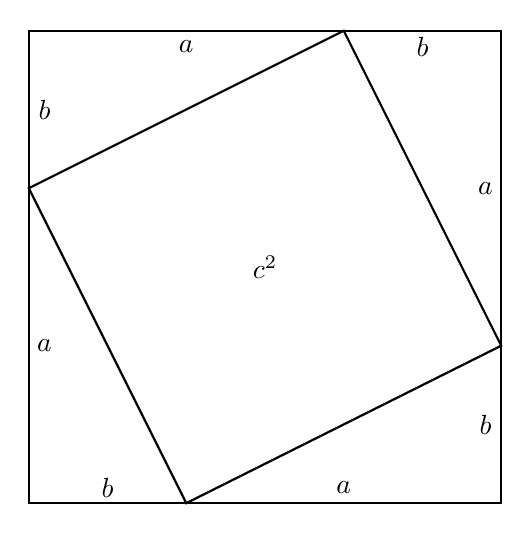
\begin{tikzpicture}
% Outer large square
\draw[thick] (0, 0) -- (6, 0) -- (6, 6) -- (0, 6) -- cycle;
% Inner smaller square
\draw[thick] (2, 0) -- (6, 2) -- (4, 6) -- (0, 4) -- cycle;

% Labels (starting from the left side and labeling the segments clockwise)
\node at (0.2, 5) {\(b\)};
\node at (5, 5.8) {\(b\)};
\node at (5.8, 1) {\(b\)};
\node at (1, 0.2) {\(b\)};

% Labels (starting from the left side and labeling the segments clockwise)
\node at (0.2, 2) {\(a\)};
\node at (2, 5.8) {\(a\)};
\node at (5.8, 4) {\(a\)};
\node at (4, 0.2) {\(a\)};

\node at (3, 3) {\(c^2\)};


\end{tikzpicture}
\end{center}

The area of the large square is:
\[
\text{Area of large square} = (a + b)^2 = a^2 + 2ab + b^2
\]

The area of the four triangles is:
\[
\text{Area of four triangles} = 4 \times \frac{1}{2}ab = 2ab
\]

The area of the inner square is:
\[
\text{Area of inner square} = c^2
\]

Now, the total area of the large square can also be written as the sum of the areas of the four triangles and the inner square:
\[
a^2 + 2ab + b^2 = 2ab + c^2
\]

Canceling \(2ab\) from both sides:
\[
a^2 + b^2 = c^2
\]

Thus, we have proven the Pythagorean theorem:
\[
c^2 = a^2 + b^2
\]

\end{document}
